\documentclass[12pt, a4paper]{article}

% --- Pakiety ---
\usepackage[utf8]{inputenc}
\usepackage[T1]{fontenc}
\usepackage[polish]{babel}
\usepackage{geometry}
\usepackage{amsmath}
\usepackage{amssymb}
\usepackage{graphicx}
\usepackage{booktabs}
\usepackage{siunitx}
\usepackage{caption}
\usepackage{subcaption}
\usepackage{float}
\usepackage{hyperref}
\usepackage{xcolor}
\usepackage{array}
\usepackage{multirow}
\usepackage{fancyhdr}

% --- Marginesy ---
\geometry{
    top=2.5cm,
    bottom=2.5cm,
    left=2.5cm,
    right=2.5cm,
    footskip=2cm
}

% --- Stopka ---
\pagestyle{fancy}
\fancyhf{}
\renewcommand{\headrulewidth}{0pt}
\renewcommand{\footrulewidth}{0.4pt}
\fancyfoot[R]{
\includegraphics[height=0.8cm]{lumon.pdf}}

% --- Konfiguracja siunitx ---
\sisetup{
    output-decimal-marker = {,},
    separate-uncertainty = true
}

% --- Dane raportu ---
\newcommand{\tytul}{Badanie widm emisyjnych za pomocą spektroskopu pryzmatycznego}
\newcommand{\codeword}{Cairns}
\newcommand{\nrCwiczenia}{O10}
\newcommand{\autor}{Karol Peszek}
\newcommand{\nrGrupy}{A}
\newcommand{\dataWykonania}{20 października 2026}

% --- Tytuł dokumentu ---
\title{
    \large I Pracownia Fizyczna \\[0.5em]
    \textbf{Ćwiczenie \nrCwiczenia} \\[0.3em]
    \LARGE \tytul\space''\codeword''
}
\author{
    \autor\\
     Grupa \nrGrupy}
\date{
    Data wykonania pomiarów: \dataWykonania\\
}

% =============================================
\begin{document}
% =============================================

\maketitle
\thispagestyle{empty}
\newpage

% -------------------------------------------
\section{Cel ćwiczenia}
% -------------------------------------------

W niniejszej pracy zbadano liniowe widma emisyjne sześciu źródeł światła: lamp
spektralnych rtęciowej, kadmowej, cynkowej i sodowej oraz rurek Geisslera z helem
i neonem. Za pomocą spektroskopu pryzmatycznego zmierzono położenia linii widmowych
na skali umownej przyrządu. Na podstawie linii helu, rtęci i kadmu o znanych długościach
fal sporządzono krzywą dyspersji spektroskopu, a następnie wyznaczono długości fal linii
cynku, sodu i neonu i porównano je z wartościami tablicowymi.

% -------------------------------------------
\section{Wstęp teoretyczny}
% -------------------------------------------

\subsection{Widma atomowe}

Atom składa się z niewielkiego, ciężkiego jądra i elektronów, których stan opisują
orbitale --- funkcje falowe będące rozwiązaniami równania Schrödingera. Energia elektronu
w atomie jest skwantowana: przyjmuje tylko wartości dyskretne, charakterystyczne dla
danego pierwiastka. Przejście elektronu z orbitalu o energii $E_p$ na orbital o niższej
energii $E_k$ wiąże się z emisją fotonu o energii~\cite{skrypt}
\begin{equation}
    E_\text{em} = E_p - E_k = h\nu,
    \label{eq:emission}
\end{equation}
gdzie $h$ --- stała Plancka, $\nu$ --- częstotliwość emitowanej fali. Długość fali
wynosi $\lambda = c/\nu$, gdzie $c$ --- prędkość światła w próżni.

Ponieważ układ poziomów energetycznych jest inny dla każdego pierwiastka, atomy
emitują charakterystyczny zestaw długości fal. Widmo pobudzonego do świecenia gazu
atomowego składa się z wyraźnie oddzielonych \emph{linii widmowych}, co pozwala
zidentyfikować skład substancji świecącej (spektralna analiza widmowa). Cząsteczki
emitują widma pasmowe, a rozżarzone ciała stałe, ciecze i gazy pod dużym ciśnieniem ---
widma ciągłe.

\subsection{Dyspersja i bieg światła w pryzmacie}

Do rozłożenia światła na składowe wykorzystuje się \emph{dyspersję} --- zależność
współczynnika załamania $n$ od długości fali. Poza obszarami pochłaniania dyspersja
jest \emph{normalna} ($n$ maleje ze wzrostem $\lambda$) i opisuje ją wzór
Cauchy'ego~\cite{skrypt}
\begin{equation}
    n = A + \frac{B}{\lambda^2},
    \label{eq:cauchy}
\end{equation}
gdzie $A$ i $B$ --- stałe charakterystyczne dla ośrodka. W obszarze pochłaniania
$n(\lambda)$ pozostaje funkcją ciągłą, ale zmienia się gwałtownie i~rośnie z~długością
fali ($\mathrm{d}n/\mathrm{d}\lambda > 0$) --- jest to obszar dyspersji \emph{anomalnej}.

Elementem dyspersyjnym spektroskopu jest szklany pryzmat. Wiązka światła załamuje się
na pierwszej ścianie pryzmatu, a ponieważ $n$ zależy od $\lambda$, każda barwa biegnie
dalej pod innym kątem. Drugie załamanie, przy wyjściu z pryzmatu, dodatkowo zwiększa
rozbieżność promieni (Rysunek~\ref{fig:prism}). Światło fioletowe, dla którego $n$
jest największe, odchyla się najsilniej.

\begin{figure}[H]
    \centering
    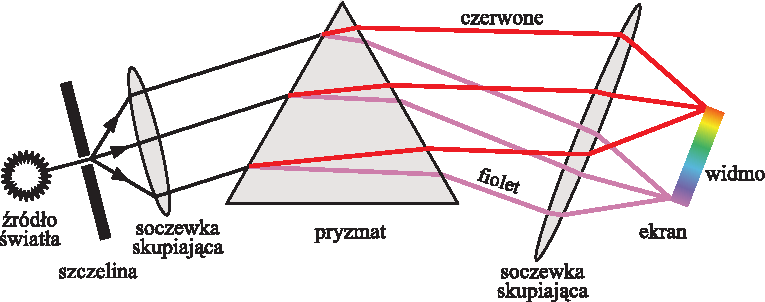
\includegraphics[width=0.75\textwidth]{prism.pdf}
    \caption{Bieg wiązki światła przez pryzmat i rozszczepienie światła białego na widmo.
             Źródło:~\cite{skrypt}.}\label{fig:prism}
\end{figure}

Oznaczenia kątów dla promienia monochromatycznego pokazano na
Rysunku~\ref{fig:prism_angles}. Z prawa Snella na obu ścianach pryzmatu~\cite{skrypt}
\begin{equation}
    n = \frac{\sin\alpha_1}{\sin\beta_1} = \frac{\sin\alpha_2}{\sin\beta_2},
    \label{eq:snell}
\end{equation}
gdzie $\alpha_1$, $\beta_2$ --- kąty padania, a $\beta_1$, $\alpha_2$ --- kąty
załamania na pierwszej i drugiej ścianie. \emph{Kąt odchylenia} $\delta$ to kąt między
kierunkiem wiązki wchodzącej i wychodzącej z pryzmatu. Z geometrii rysunku
\begin{equation}
    \varphi = \beta_1 + \beta_2, \qquad
    \delta = (\alpha_1 - \beta_1) + (\alpha_2 - \beta_2) = \alpha_1 + \alpha_2 - \varphi,
    \label{eq:deviation}
\end{equation}
gdzie $\varphi$ --- kąt łamiący pryzmatu. Kąt $\delta$ zależy od kąta padania $\alpha_1$
i osiąga minimum $\delta_m$ (\emph{kąt najmniejszego odchylenia}), gdy promień biegnie
przez pryzmat symetrycznie ($\alpha_1 = \alpha_2$). W tym położeniu $\delta$ najsłabiej
zależy od niewielkich zmian kąta padania, dlatego pryzmat spektroskopu ustawia się na
kąt najmniejszego odchylenia.

\begin{figure}[H]
    \centering
    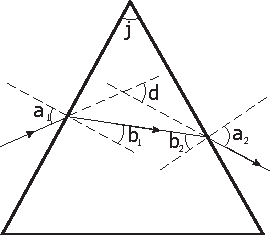
\includegraphics[width=0.35\textwidth]{prism_angles.pdf}
    \caption{Zależności kątowe przy załamaniu światła monochromatycznego w pryzmacie
             o kącie łamiącym $\varphi$; $\delta$ --- kąt odchylenia.
             Źródło:~\cite{skrypt}.}\label{fig:prism_angles}
\end{figure}

\subsection{Krzywa dyspersji}

Podstawienie zależności~\eqref{eq:deviation} do~\eqref{eq:snell} daje~\cite{skrypt}
\begin{equation}
    n = \frac{\sin\alpha_1}{\sin(\varphi - \alpha_1)}
      = \frac{\sin\delta\cos(\varphi - \alpha_1) + \cos\delta\sin(\varphi - \alpha_1)}
             {\sin(\varphi - \alpha_1)}.
    \label{eq:n_delta}
\end{equation}
Kąt odchylenia dla danej długości fali zapisuje się jako $\delta = \delta_m + \gamma$.
Dla małego $\gamma$ można rozwinąć $\sin(\delta_m + \gamma) \approx \sin\delta_m +
\gamma\cos\delta_m$ i $\cos(\delta_m + \gamma) \approx \cos\delta_m - \gamma\sin\delta_m$,
skąd współczynnik załamania jest liniową funkcją $\gamma$: $n = p_1 + q_1\gamma$.
W przybliżeniu małych kątów położenie linii $x$ na skali spektroskopu jest liniową funkcją
$\gamma$, $x = x_0 + k\gamma$ (zero skali nie musi odpowiadać $\gamma = 0$; przesunięcie $x_0$
pochłania wyraz stały), zatem $n = p_2 + q_2 x$, gdzie $p_1, q_1, p_2, q_2, x_0, k$ --- stałe układu.
Porównanie ze wzorem Cauchy'ego~\eqref{eq:cauchy} prowadzi do liniowej zależności
odwrotności kwadratu długości fali od położenia linii~\cite{skrypt}:
\begin{equation}
    \frac{1}{\lambda^2} = a_1 + a_2 x,
    \label{eq:dispersion_linear}
\end{equation}
gdzie $a_1$ --- wartość $1/\lambda^2$ odpowiadająca zeru skali, $a_2$ --- przyrost
$1/\lambda^2$ na jedną działkę skali.

Wzór~\eqref{eq:dispersion_linear} wynika z trzech przybliżeń: rozwinięcia funkcji
trygonometrycznych do pierwszego rzędu w $\gamma$, liniowości odwzorowania kąta $\gamma$
na położenie $x$ oraz dwuwyrazowego wzoru Cauchy'ego (z pominięciem wyrazu $C/\lambda^4$).
Na całym zakresie widzialnym każde z nich może dawać mierzalną poprawkę drugiego rzędu.
Najprostsze rozszerzenie modelu ma postać
\begin{equation}
    \frac{1}{\lambda^2} = a_1 + a_2 x + a_3 x^2,
    \label{eq:dispersion_quadratic}
\end{equation}
gdzie $a_3$ --- współczynnik opisujący odstępstwo od liniowości. Zależność $\lambda(x)$,
wyznaczona dla linii o znanych długościach fal, jest \emph{krzywą dyspersji}
(krzywą kalibracyjną) spektroskopu: pozwala przypisać długość fali dowolnej linii na
podstawie jej położenia na skali.

\subsection{Spektroskop pryzmatyczny}

Spektroskop składa się z kolimatora~K, pryzmatu i lunety~L
(Rysunek~\ref{fig:spectroscope_scheme}). Kolimator ma na wejściu szczelinę o regulowanej
szerokości, umieszczoną w ognisku jego soczewki, dzięki czemu na pryzmat pada wiązka
równoległa i wszystkie promienie padają pod tym samym kątem. Po przejściu przez pryzmat
światło trafia do lunety, w której obserwuje się obraz szczeliny w tylu barwach, ile
długości fal zawiera światło padające na szczelinę~\cite{skrypt}.

Aby przyrząd umożliwiał odczyt położenia linii, wyposażono go w dodatkowy kolimator~L$_1$
z podziałką liniową niemianowaną (skalą umowną). Obraz skali, oświetlonej osobną lampą,
odbija się od ściany pryzmatu i trafia do lunety razem z widmem, więc położenie każdej
linii można odczytać bezpośrednio na skali~\cite{skrypt}.

\begin{figure}[H]
    \centering
    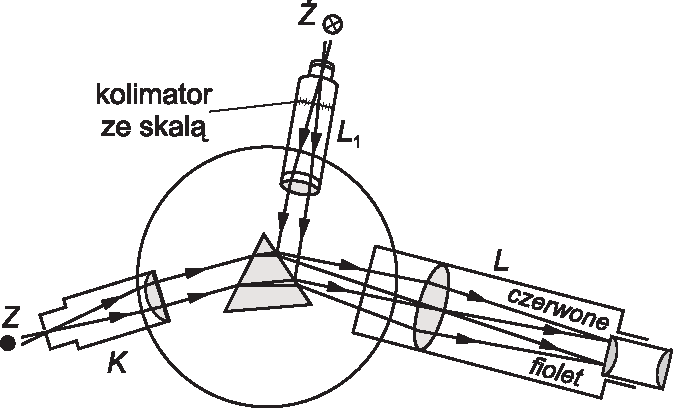
\includegraphics[width=0.72\textwidth]{schema.pdf}
    \caption{Schemat spektroskopu pryzmatycznego: Z --- źródło światła, K --- kolimator
             ze szczeliną, L --- luneta, L$_1$ --- kolimator ze skalą oświetlany źródłem Ż.
             Źródło:~\cite{skrypt}.}\label{fig:spectroscope_scheme}
\end{figure}

\subsection{Wartości tablicowe}

Długości fal linii wzorcowych (He, Hg, Cd) oraz linii użytych do porównania (Zn, Na, Ne)
przyjęto z bazy NIST Atomic Spectra Database~\cite{nist}. Ponieważ pomiar odbywał się
w powietrzu, użyto obserwowanych długości fal w powietrzu, podawanych dalej z~dokładnością
do $0{,}001$~nm. Linie, których składowych spektroskop nie
rozdziela (żółty dublet rtęci $576{,}96$ / $579{,}07$~nm oraz dublety sodu), opisano
średnią długością fali składowych z niepewnością równą połowie ich odstępu.

% -------------------------------------------
\section{Opis układu pomiarowego}
% -------------------------------------------

Układ pomiarowy przedstawiono na Rysunku~\ref{fig:setup}. Przed szczeliną kolimatora
spektroskopu ustawiano kolejno badane źródła światła; na zdjęciu przed szczeliną stoi
lampa sodowa, a w tle lampy kadmowa i cynkowa.

\begin{figure}[H]
    \centering
    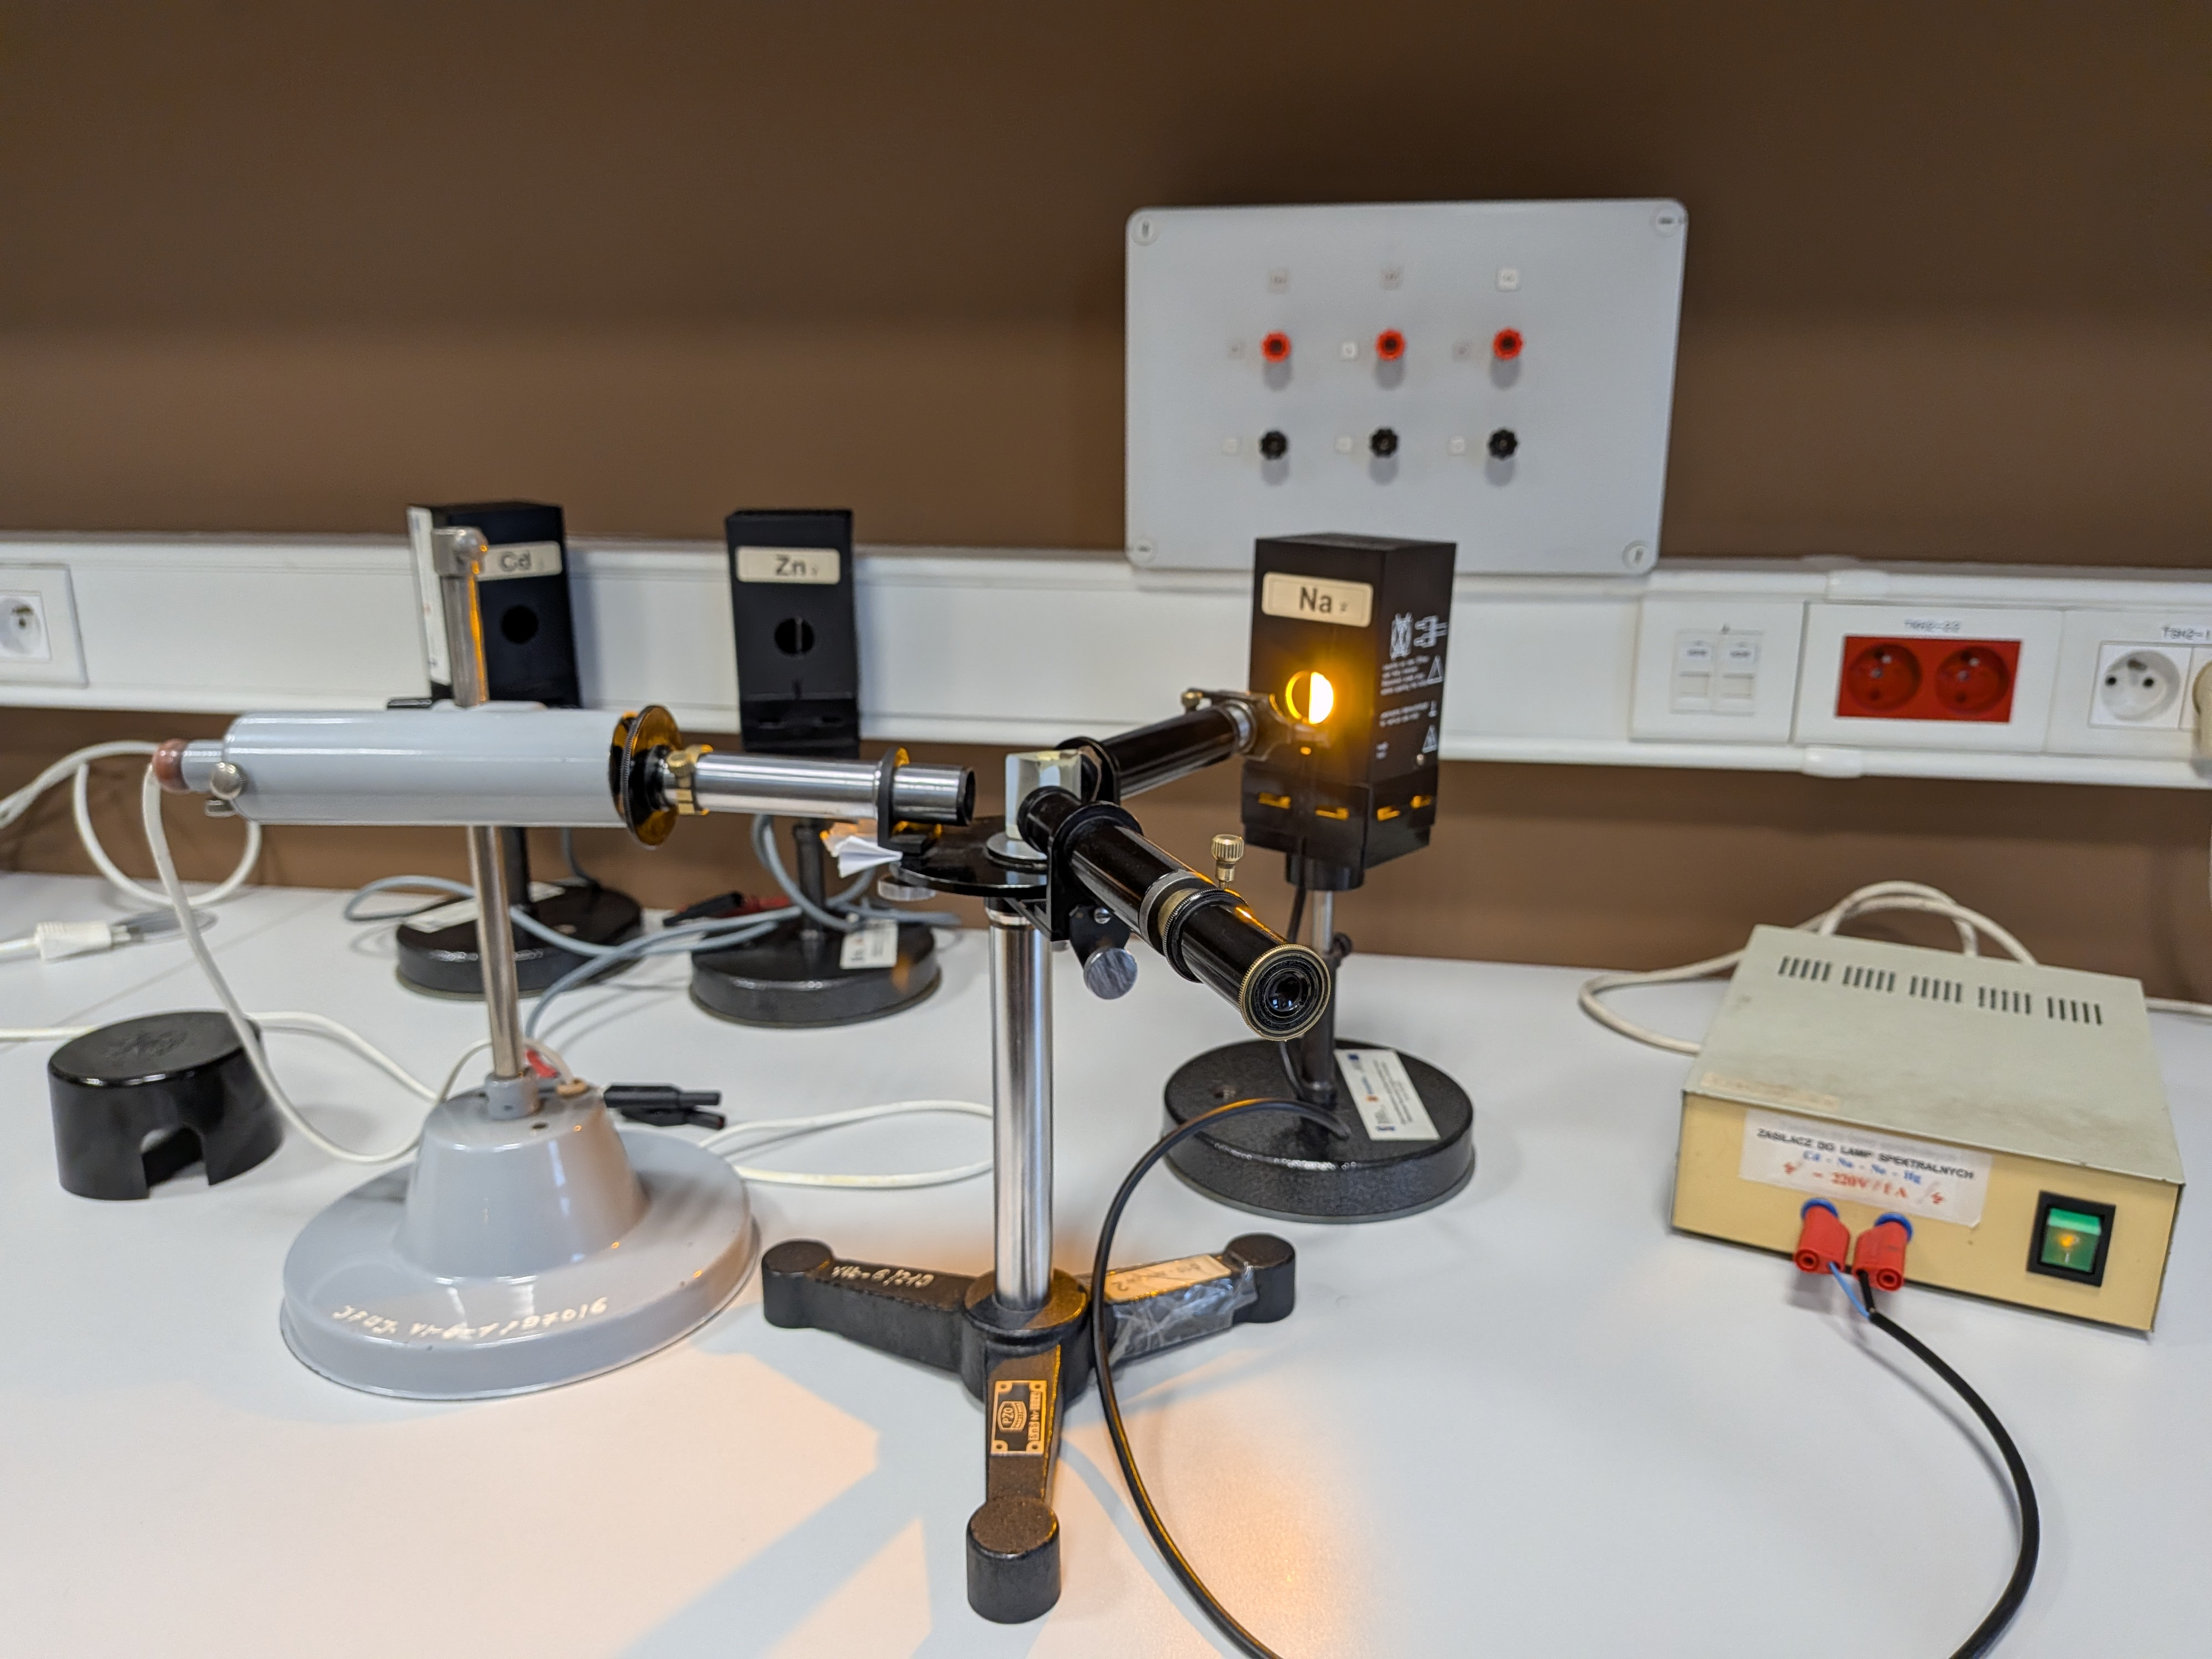
\includegraphics[width=0.82\textwidth]{schema.jpg}
    \caption{Układ pomiarowy: spektroskop pryzmatyczny na statywie, przed jego szczeliną
             lampa sodowa (Na), w tle lampy kadmowa (Cd) i cynkowa (Zn), po prawej
             zasilacz lamp spektralnych.}\label{fig:setup}
\end{figure}

W skład układu wchodziły:
\begin{itemize}
    \item spektroskop pryzmatyczny z kolimatorem ze szczeliną o regulowanej szerokości,
          pryzmatem szklanym i lunetą z krzyżem z nici pajęczych,
    \item kolimator ze skalą umowną \numrange{0}{20}~działek [dz.], podzielonych na
          dziesiąte części, oświetlany osobną lampą; niepewność odczytu położenia linii
          $u_x = 0{,}2$~dz. (paralaksa, skończona szerokość obrazu szczeliny i ocena
          środka linii okiem),
    \item lampy spektralne: rtęciowa (Hg), kadmowa (Cd), cynkowa (Zn) i sodowa (Na)
          wraz z zasilaczem,
    \item rurki Geisslera z helem (He) i neonem (Ne) wraz z zasilaczem.
\end{itemize}

Światło badanego źródła oświetlało szczelinę kolimatora~K, a światło lampy oświetlającej
skalę --- kolimator~L$_1$. W polu widzenia lunety obserwowano jednocześnie obraz szczeliny
w barwach linii widmowych i obraz skali, odbity od ściany pryzmatu
(Rysunek~\ref{fig:spectroscope_scheme}).



% -------------------------------------------
\section{Procedura pomiarowa}
% -------------------------------------------

\subsection{Justowanie spektroskopu}

Lunetę ustawiono „na nieskończoność”, ogniskując ją na odległy przedmiot, a następnie
okularem ustawiono ostry obraz krzyża z nici pajęczych i sprawdzono brak paralaksy
(krzyż nie przesuwał się względem obrazu przy ruchu oka w bok). Kolimator ustawiono
współosiowo z lunetą i oświetlono szczelinę lampą sodową. Odległość szczeliny od soczewki
kolimatora dobrano tak, aby obraz szczeliny w lunecie był ostry i pionowy, a szerokość
szczeliny --- tak, aby obraz był wąski, ale wyraźny. Od tego momentu nie zmieniano
ustawienia lunety ani kolimatora; w trakcie pomiarów regulowano jedynie szerokość
szczeliny, aby słabe linie były widoczne.

\subsection{Ustawienie pryzmatu na kąt najmniejszego odchylenia}

Pryzmat zamocowano na stoliku spektroskopu i odnaleziono w lunecie obraz szczeliny
utworzony przez promienie odchylone w pryzmacie. Obracano pryzmat, obserwując przesuwanie
się obrazu szczeliny w polu widzenia. Pryzmat zostawiono w położeniu „punktu zwrotnego”,
w którym obraz szczeliny, mimo dalszego obrotu pryzmatu w tę samą stronę, zaczynał
przesuwać się w przeciwnym kierunku --- odpowiada ono kątowi najmniejszego odchylenia
$\delta_m$. Następnie oświetlono kolimator ze skalą i ustawiono go tak, aby w lunecie
widoczny był ostry obraz skali obok widma.

\subsection{Pomiar położeń linii widmowych}

Przed szczeliną kolimatora umieszczano kolejno źródła światła: lampy spektralne rtęciową,
kadmową, cynkową i sodową oraz rurki Geisslera z helem i neonem. Procedura była dla
wszystkich źródeł taka sama. Po włączeniu lampy i ustabilizowaniu się jej świecenia
przesuwano wzrok wzdłuż widma od strony czerwonej do fioletowej i dla każdej widocznej
linii zapisywano:
\begin{itemize}
    \item położenie linii na skali umownej $x$, odczytane z rozdzielczością $0{,}1$~dz.,
    \item barwę linii,
    \item ocenę jasności linii w umownej skali od 1 (linia na granicy widoczności)
          do 10 (najjaśniejsza linia).
\end{itemize}
Każdy odczyt zapisywano od razu, osobno dla każdej linii, tak aby powstał komplet danych
dla całego widma przed zmianą źródła. Linie leżące poza końcem podziałki
(dwie najbardziej fioletowe linie sodu) zanotowano z położeniem oszacowanym przez
przedłużenie skali i oznaczono jako szacunkowe.



% -------------------------------------------
\section{Wyniki pomiarów}
% -------------------------------------------

We wszystkich pomiarach niepewność odczytu położenia linii na skali wynosi
$u_x = 0{,}2$~dz. Jasność linii oceniano subiektywnie w umownej skali od 1 do 10.

\subsection{Pomiar położeń linii widmowych}

Łącznie zanotowano 70 linii widmowych: 10 dla helu, 4 dla rtęci, 10 dla kadmu, 8 dla
cynku, 14 dla sodu i 24 dla neonu. Obserwowane widma wszystkich źródeł zestawiono na
Rysunku~\ref{fig:spectra_raw}, a zanotowane położenia, barwy i jasności linii --- w
Tabelach~\ref{tab:raw_he}--\ref{tab:raw_ne}. Barwy podano tak, jak zostały zapisane
podczas pomiaru. Dwie ostatnie linie sodu leżą poza końcem podziałki i ich położenie
jest szacunkowe.

\begin{figure}[H]
    \centering
    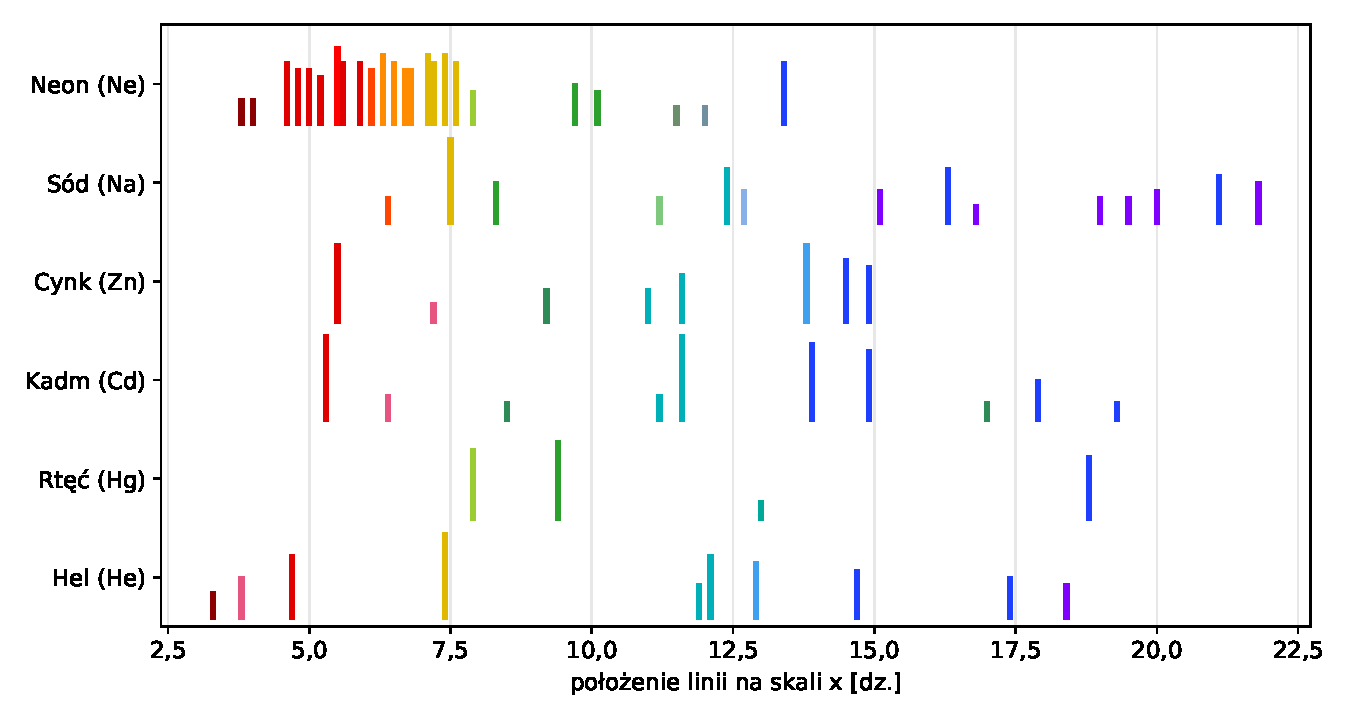
\includegraphics[width=0.95\textwidth]{spectra_raw.pdf}
    \caption{Obserwowane widma emisyjne na skali umownej spektroskopu. Każda linia
             widmowa zaznaczona jest pionową kreską o wysokości proporcjonalnej do
             ocenionej jasności i kolorze odpowiadającym zanotowanej barwie. Niepewność
             położenia każdej linii wynosi $u_x = 0{,}2$~dz.}\label{fig:spectra_raw}
\end{figure}

\begin{table}[H]
    \centering
    \caption{Położenia $x$, barwy i jasności linii widmowych helu (He, rurka Geisslera).}\label{tab:raw_he}
    \begin{tabular}{c S[table-format=2.1] S[table-format=2.0] l}
        \toprule
        Nr & {$x$ [dz.]} & {jasność} & barwa \\
        \midrule
        1 & 3.3 & 2 & ciemnoczerwony (bardzo słaby) \\
        2 & 3.8 & 4 & różowoczerwony \\
        3 & 4.7 & 7 & czerwony \\
        4 & 7.4 & 10 & żółty \\
        5 & 11.9 & 3 & zielononiebieski (cyjan) \\
        6 & 12.1 & 7 & zielononiebieski (cyjan) \\
        7 & 12.9 & 6 & błękitny \\
        8 & 14.7 & 5 & niebieski \\
        9 & 17.4 & 4 & niebieski / indygo \\
        10 & 18.4 & 3 & fioletowoniebieski \\
        \bottomrule
    \end{tabular}
\end{table}

\begin{table}[H]
    \centering
    \caption{Położenia $x$, barwy i jasności linii widmowych lampy rtęciowej (Hg).}\label{tab:raw_hg}
    \begin{tabular}{c S[table-format=2.1] S[table-format=2.0] l}
        \toprule
        Nr & {$x$ [dz.]} & {jasność} & barwa \\
        \midrule
        1 & 7.9 & 8 & żółtozielony \\
        2 & 9.4 & 9 & zielony \\
        3 & 13.0 & 1 & błękitnozielony (bardzo słaby) \\
        4 & 18.8 & 7 & niebieski \\
        \bottomrule
    \end{tabular}
\end{table}

\begin{table}[H]
    \centering
    \caption{Położenia $x$, barwy i jasności linii widmowych lampy kadmowej (Cd).}\label{tab:raw_cd}
    \begin{tabular}{c S[table-format=2.1] S[table-format=2.0] l}
        \toprule
        Nr & {$x$ [dz.]} & {jasność} & barwa \\
        \midrule
        1 & 5.3 & 10 & czerwony \\
        2 & 6.4 & 2 & różowoczerwony (słaby) \\
        3 & 8.5 & 1 & morskozielony (bardzo słaby) \\
        4 & 11.2 & 2 & cyjan (słaby) \\
        5 & 11.6 & 10 & cyjan \\
        6 & 13.9 & 9 & niebieski \\
        7 & 14.9 & 8 & niebieski \\
        8 & 17.0 & 1 & morskozielony (bardzo słaby) \\
        9 & 17.9 & 4 & niebieskofioletowy \\
        10 & 19.3 & 1 & niebieski (bardzo słaby) \\
        \bottomrule
    \end{tabular}
\end{table}

\begin{table}[H]
    \centering
    \caption{Położenia $x$, barwy i jasności linii widmowych lampy cynkowej (Zn).}\label{tab:raw_zn}
    \begin{tabular}{c S[table-format=2.1] S[table-format=2.0] l}
        \toprule
        Nr & {$x$ [dz.]} & {jasność} & barwa \\
        \midrule
        1 & 5.5 & 9 & czerwony \\
        2 & 7.2 & 1 & różowawy (bardzo słaby) \\
        3 & 9.2 & 3 & morskozielony \\
        4 & 11.0 & 3 & cyjan \\
        5 & 11.6 & 5 & cyjan \\
        6 & 13.8 & 9 & jasny błękitny \\
        7 & 14.5 & 7 & niebieski \\
        8 & 14.9 & 6 & niebieski \\
        \bottomrule
    \end{tabular}
\end{table}

\begin{table}[H]
    \centering
    \caption{Położenia $x$, barwy i jasności linii widmowych lampy sodowej (Na).}\label{tab:raw_na}
    \begin{tabular}{c S[table-format=2.1] S[table-format=2.0] l}
        \toprule
        Nr & {$x$ [dz.]} & {jasność} & barwa \\
        \midrule
        1 & 6.4 & 2 & pomarańczowoczerwony (słaby) \\
        2 & 7.5 & 10 & żółty \\
        3 & 8.3 & 4 & zielony \\
        4 & 11.2 & 2 & bladozielony \\
        5 & 12.4 & 6 & cyjan \\
        6 & 12.7 & 3 & bladoniebieski \\
        7 & 15.1 & 3 & fioletowoniebieski (słaby) \\
        8 & 16.3 & 6 & niebieski \\
        9 & 16.8 & 1 & fioletowoniebieski (bardzo słaby) \\
        10 & 19.0 & 2 & fioletowy (słaby) \\
        11 & 19.5 & 2 & fioletowy (słaby) \\
        12 & 20.0 & 3 & fioletowy \\
        13 & 21.1 & 5 & niebieskofioletowy (poza skalą, szacunkowo) \\
        14 & 21.8 & 4 & fioletowy (poza skalą, szacunkowo) \\
        \bottomrule
    \end{tabular}
\end{table}

\begin{table}[H]
    \centering
    \caption{Położenia $x$, barwy i jasności linii widmowych neonu (Ne, rurka Geisslera).}\label{tab:raw_ne}
    \begin{tabular}{c S[table-format=2.1] S[table-format=2.0] l}
        \toprule
        Nr & {$x$ [dz.]} & {jasność} & barwa \\
        \midrule
        1 & 3.8 & 2 & ciemnoczerwony / purpurowy \\
        2 & 4.0 & 2 & ciemnoczerwony / purpurowy \\
        3 & 4.6 & 7 & czerwony \\
        4 & 4.8 & 6 & czerwony \\
        5 & 5.0 & 6 & czerwony \\
        6 & 5.2 & 5 & czerwony \\
        7 & 5.5 & 9 & jaskrawoczerwony \\
        8 & 5.6 & 7 & czerwony \\
        9 & 5.9 & 7 & czerwony \\
        10 & 6.1 & 6 & czerwono-pomarańczowy \\
        11 & 6.3 & 8 & pomarańczowy \\
        12 & 6.5 & 7 & pomarańczowy \\
        13 & 6.7 & 6 & pomarańczowy \\
        14 & 6.8 & 6 & pomarańczowo-żółty \\
        15 & 7.1 & 8 & żółto-pomarańczowy \\
        16 & 7.2 & 7 & żółty \\
        17 & 7.4 & 8 & żółty \\
        18 & 7.6 & 7 & żółty \\
        19 & 7.9 & 3 & żółtozielony \\
        20 & 9.7 & 4 & zielony \\
        21 & 10.1 & 3 & zielony \\
        22 & 11.5 & 1 & szarozielony (bardzo słaby) \\
        23 & 12.0 & 1 & szaroniebieskawy (bardzo słaby) \\
        24 & 13.4 & 7 & niebieski \\
        \bottomrule
    \end{tabular}
\end{table}


% -------------------------------------------
\section{Opracowanie wyników}
% -------------------------------------------

\subsection{Odrzucenie linii}

Z dalszej analizy odrzucono 10 z~70 zanotowanych linii. Osiem z~nich (Ne~22, Ne~23,
Hg~3, Na~9, Zn~2, Cd~3, Cd~8, Cd~10) oceniono na jasność 1 --- ich obraz był na granicy
widoczności i nie dało się pewnie wskazać środka linii, więc niepewność $u_x = 0{,}2$~dz.
nie opisuje błędu ich odczytu. Dwie linie sodu (Na~13 i Na~14) leżały poza podziałką,
a ich położenie było jedynie szacowane.

\subsection{Krzywa dyspersji}\label{sec:dispersion_fit}

Do wyznaczenia krzywej dyspersji wybrano hel, rtęć i~kadm: ich linie mają jednoznaczne
odpowiedniki w~bazie NIST~\cite{nist} i~pokrywają zakres skali od $3{,}3$ do $18{,}8$~dz.
Przypisano 18 linii (Tabela~\ref{tab:calibration}): 10 linii He~I, 3 linie Hg~I
(w tym nierozdzielony żółty dublet) oraz 4 linie Cd~I i~jedną linię jonu Cd~II
($441{,}569$~nm). Dwie słabe linie lampy kadmowej (Cd~2 i~Cd~4, jasność 2) nie weszły
do kalibracji: dla Cd~2 przypisanie linii Cd~I jest niejednoznaczne, a obie leżą w~położeniach
linii sodu. Omówiono je w~p.~\ref{sec:nist}.

\begin{table}[H]
    \centering
    \caption{Linie wzorcowe użyte do kalibracji: położenie $x$, długość fali z~NIST~\cite{nist} $\lambda_\text{NIST}$ oraz długości fal odtworzone z~modelu liniowego $\lambda_\text{lin}$ i~kwadratowego $\lambda_\text{kw}$. Dla linii Hg~1 (nierozdzielony dublet) $u_\lambda = 1{,}05$~nm.}\label{tab:calibration}
    \begin{tabular}{c c S[table-format=2.1] S[table-format=3.3] S[table-format=3.1] S[table-format=3.1]}
        \toprule
        Źródło & Nr & {$x$ [dz.]} & {$\lambda_\text{NIST}$ [nm]} & {$\lambda_\text{lin}$ [nm]} & {$\lambda_\text{kw}$ [nm]} \\
        \midrule
        He & 1 & 3.3 & 728.135 & 711.7 & 729.6 \\
        He & 2 & 3.8 & 706.519 & 692.8 & 705.6 \\
        He & 3 & 4.7 & 667.815 & 662.2 & 668.3 \\
        He & 4 & 7.4 & 587.562 & 590.1 & 586.8 \\
        He & 5 & 11.9 & 504.774 & 509.2 & 504.9 \\
        He & 6 & 12.1 & 501.568 & 506.4 & 502.1 \\
        He & 7 & 12.9 & 492.193 & 495.4 & 491.8 \\
        He & 8 & 14.7 & 471.315 & 473.1 & 471.3 \\
        He & 9 & 17.4 & 447.148 & 444.6 & 446.4 \\
        He & 10 & 18.4 & 438.793 & 435.3 & 438.5 \\
        Hg & 1 & 7.9 & 578.014 & 579.2 & 575.2 \\
        Hg & 2 & 9.4 & 546.075 & 549.7 & 544.7 \\
        Hg & 4 & 18.8 & 435.834 & 431.7 & 435.6 \\
        Cd & 1 & 5.3 & 643.847 & 643.9 & 646.8 \\
        Cd & 5 & 11.6 & 508.582 & 513.6 & 509.1 \\
        Cd & 6 & 13.9 & 479.991 & 482.6 & 480.0 \\
        Cd & 7 & 14.9 & 467.815 & 470.8 & 469.2 \\
        Cd & 9 & 17.9 & 441.569 & 439.8 & 442.4 \\
        \bottomrule
    \end{tabular}
\end{table}

Do punktów $(x_i,\, y_i = 1/\lambda_i^2)$ dopasowano model liniowy~\eqref{eq:dispersion_linear}
i~kwadratowy~\eqref{eq:dispersion_quadratic}, wyrażając $y$ w~\si{\micro\meter^{-2}}.
Niepewność ma głównie położenie $x$, a nie dopasowywana wielkość $y$, dlatego zastosowano
metodę wariancji efektywnej --- niepewność $u_x$ przeniesiono na oś $y$ przez nachylenie
krzywej:
\begin{equation}
    \sigma_{y,i}^2 = \left(f'(x_i)\, u_x\right)^2 + \left(\frac{2}{\lambda_i^3}\, u_{\lambda,i}\right)^2,
    \label{eq:effective_variance}
\end{equation}
gdzie $f'(x)$ --- pochodna dopasowywanej funkcji ($a_2$ dla modelu liniowego,
$a_2 + 2a_3x$ dla kwadratowego), $u_{\lambda,i}$ --- niepewność wartości tablicowej
(niezerowa tylko dla dubletu Hg). Ponieważ $\sigma_{y,i}$ zależy od parametrów,
dopasowanie wykonano iteracyjnie aż do zbieżności, za pomocą
\texttt{scipy.optimize.curve\_fit} z~argumentami \texttt{sigma}~$= \sigma_y$
i~\texttt{absolute\_sigma=True}. Niepewności parametrów obliczono jako
$u_{a_i} = \sqrt{C_{ii}}$, gdzie $C$ --- macierz kowariancji. Wyniki zestawiono
w~Tabeli~\ref{tab:fit_params}, a dopasowane krzywe i~residua pokazano na
Rysunku~\ref{fig:inverse_square}.

\begin{table}[H]
    \centering
    \caption{Parametry dopasowania modeli~\eqref{eq:dispersion_linear}
             i~\eqref{eq:dispersion_quadratic} do 18 linii wzorcowych;
             $\nu$ --- liczba stopni swobody.}\label{tab:fit_params}
    \begin{tabular}{l c c}
        \toprule
        & model liniowy & model kwadratowy \\
        \midrule
        $a_1$ [\si{\micro\meter^{-2}}]        & $1{,}252 \pm 0{,}026$   & $0{,}986 \pm 0{,}057$ \\
        $a_2$ [\si{\micro\meter^{-2}}/dz.]    & $0{,}2188 \pm 0{,}0021$ & $0{,}279 \pm 0{,}011$ \\
        $a_3$ [\si{\micro\meter^{-2}}/dz.$^2$] & ---                    & $(-2{,}74 \pm 0{,}46)\cdot 10^{-3}$ \\
        $\chi^2$                              & $34{,}6$                & $1{,}92$ \\
        $\nu$                                 & 16                      & 15 \\
        $\chi^2/\nu$                          & $2{,}16$                & $0{,}13$ \\
        \bottomrule
    \end{tabular}
\end{table}

\begin{figure}[H]
    \centering
    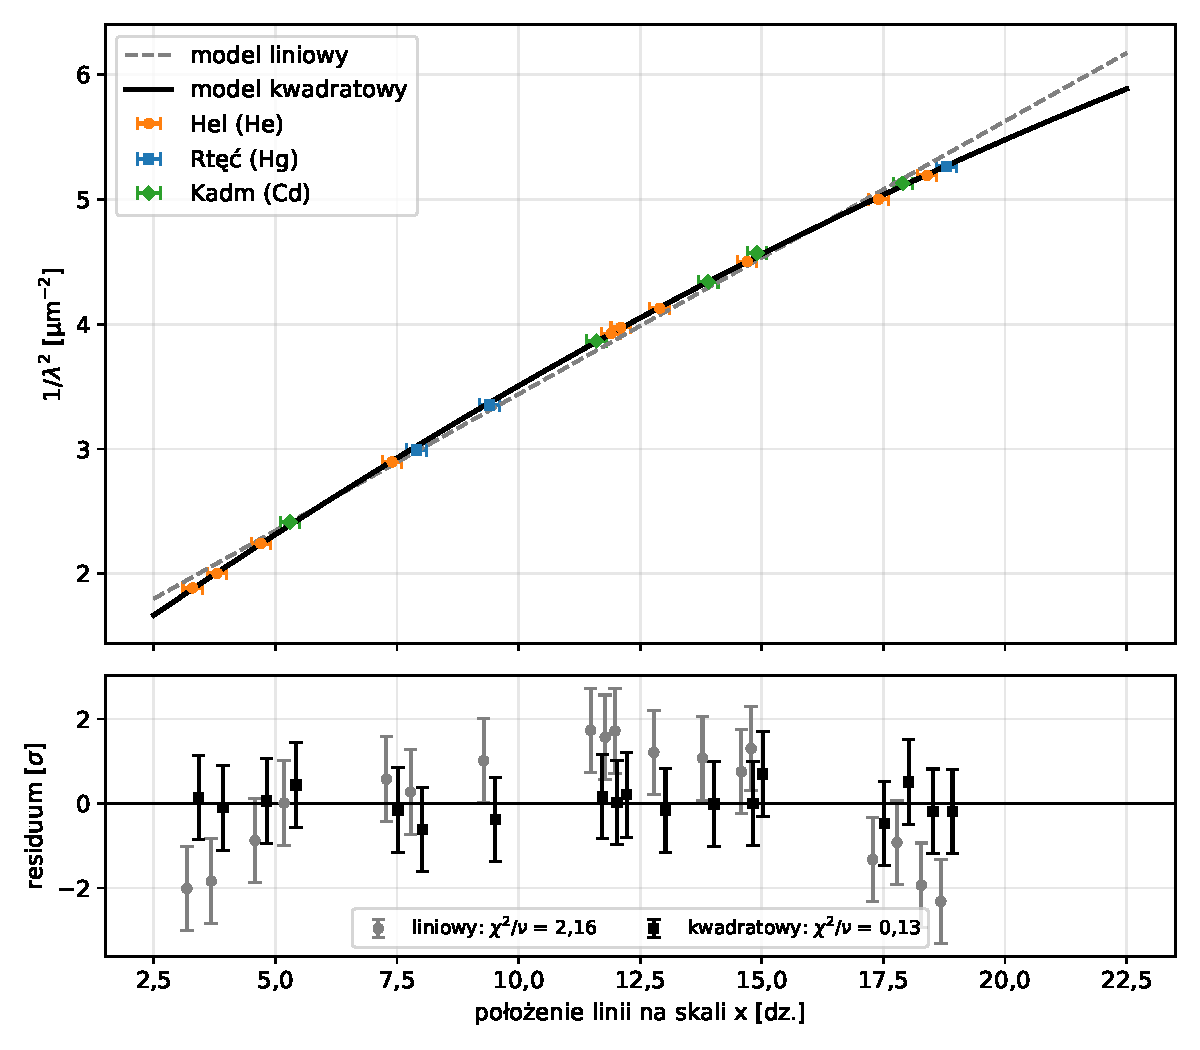
\includegraphics[width=0.78\textwidth]{inverse_square.pdf}
    \caption{Górny panel: odwrotność kwadratu długości fali linii wzorcowych w~funkcji
             położenia na skali wraz z~dopasowanym modelem liniowym (linia przerywana)
             i~kwadratowym (linia ciągła). Dolny panel: residua znormalizowane
             $(y_i - f(x_i))/\sigma_{y,i}$ dla obu modeli (punkty rozsunięte w~poziomie
             dla czytelności). Słupki błędów odpowiadają $u_x = 0{,}2$~dz.
             (górny panel) i~$1\sigma$ (dolny panel).}\label{fig:inverse_square}
\end{figure}

Model liniowy nie opisuje danych: $\chi^2 = 34{,}6$ przy $\nu = 16$ odpowiada
prawdopodobieństwu $p \approx 0{,}004$, a residua układają się w~łuk --- są ujemne na
obu końcach skali i~dodatnie w~środku. Największa rozbieżność występuje dla linii
He~1: model liniowy odtwarza ją jako $711{,}7$~nm zamiast $728{,}135$~nm
(Tabela~\ref{tab:calibration}). Dodanie wyrazu kwadratowego usuwa tę strukturę:
$a_3$ różni się od zera o $|a_3|/u(a_3) \approx 6{,}0$, co jest statystycznie istotne.
Jako krzywą kalibracyjną przyjęto więc model kwadratowy (Rysunek~\ref{fig:dispersion_curve}).

\begin{figure}[H]
    \centering
    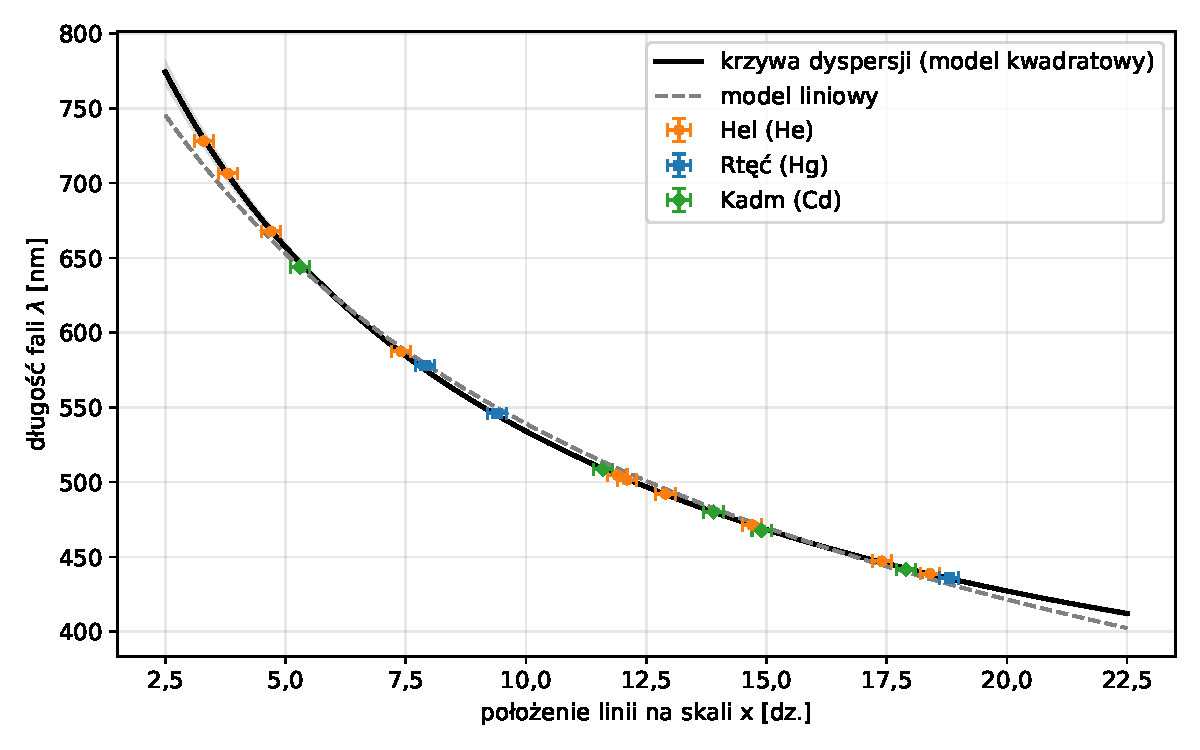
\includegraphics[width=0.78\textwidth]{dispersion_curve.pdf}
    \caption{Krzywa dyspersji spektroskopu $\lambda(x) = (a_1 + a_2x + a_3x^2)^{-1/2}$
             (linia ciągła) z~pasmem $\pm u(\lambda)$ wynikającym z~niepewności parametrów,
             model liniowy (linia przerywana) i~linie wzorcowe He, Hg i~Cd. Słupki błędów
             odpowiadają $u_x = 0{,}2$~dz. i~$u_\lambda$ wartości tablicowej.}\label{fig:dispersion_curve}
\end{figure}

Dla modelu kwadratowego $\chi^2/\nu = 0{,}13 \ll 1$. Średnie kwadratowe odchylenie punktów
od krzywej, przeliczone na położenie, wynosi $0{,}066$~dz., czyli około trzykrotnie
mniej niż przyjęta niepewność $u_x = 0{,}2$~dz. Przyjęta wartość $u_x$ jest więc
zachowawcza, a niepewności parametrów i~wyznaczanych dalej długości fal są zawyżone.
Parametry modelu kwadratowego są silnie skorelowane (współczynnik korelacji $a_2$ i~$a_3$
wynosi $-0{,}98$), dlatego w~rachunku niepewności uwzględniono pełną macierz kowariancji.

\subsection{Wyznaczenie długości fal --- linie cynku}

Długość fali linii o położeniu $x_0$ obliczono z~krzywej dyspersji:
\begin{equation}
    \lambda = \left(a_1 + a_2x_0 + a_3x_0^2\right)^{-1/2}.
    \label{eq:lambda_from_x}
\end{equation}
Niepewność $y_0 = 1/\lambda^2$ wyznaczono z~prawa propagacji niepewności, uwzględniając
kowariancję parametrów i~niepewność odczytu położenia badanej linii:
\begin{equation}
    u^2(y_0) = \sum_{i,j} \frac{\partial y_0}{\partial a_i}\frac{\partial y_0}{\partial a_j}\,C_{ij}
               + \left(\frac{\partial y_0}{\partial x_0}\, u_x\right)^2,
    \qquad
    u(\lambda) = \left|\frac{\mathrm{d}\lambda}{\mathrm{d}y_0}\right| u(y_0) = \frac{\lambda^3}{2}\, u(y_0),
    \label{eq:lambda_uncertainty}
\end{equation}
gdzie $\partial y_0/\partial a_i = x_0^{\,i-1}$ i~$\partial y_0/\partial x_0 = a_2 + 2a_3x_0$.
Dominującym źródłem niepewności jest odczyt położenia: dla linii cynku człon z~$u_x$
odpowiada za $88$--$91\,\%$ wariancji $u^2(\lambda)$. Ponieważ krzywa dyspersji
jest płaska w~czerwieni, ta sama niepewność $u_x$ daje tam większe $u(\lambda)$:
$|\mathrm{d}\lambda/\mathrm{d}x|$ wynosi $33$~nm/dz. dla $x = 5{,}5$~dz.
i~$10$~nm/dz. dla $x = 14{,}9$~dz.

Lampy cynkowej nie użyto do kalibracji, więc jej linie stanowią niezależny test krzywej
dyspersji. Wyniki dla pięciu linii Zn~I zestawiono w~Tabeli~\ref{tab:zinc}. Zgodność
oceniono testem $3\sigma$, $z = |\lambda - \lambda_\text{NIST}|/u(\lambda)$.

\begin{table}[H]
    \centering
    \caption{Długości fal linii cynku wyznaczone z~modelu liniowego ($\lambda_\text{lin}$) i~kwadratowego ($\lambda_\text{kw}$), porównane z~wartościami NIST~\cite{nist}; $z = |\lambda - \lambda_\text{NIST}|/u(\lambda)$.}\label{tab:zinc}
    \begin{tabular}{c S[table-format=2.1] S[table-format=3.3] S[table-format=3.1]@{\,$\pm$\,}S[table-format=1.1] S[table-format=1.2] S[table-format=3.1]@{\,$\pm$\,}S[table-format=1.1] S[table-format=1.2]}
        \toprule
        Nr & {$x$ [dz.]} & {$\lambda_\text{NIST}$ [nm]} & \multicolumn{2}{c}{$\lambda_\text{lin}$ [nm]} & {$z_\text{lin}$} & \multicolumn{2}{c}{$\lambda_\text{kw}$ [nm]} & {$z_\text{kw}$} \\
        \midrule
        1 & 5.5 & 636.235 & 638.1 & 6.1 & 0.32 & 640.2 & 7.0 & 0.56 \\
        4 & 11.0 & 518.198 & 522.8 & 3.2 & 1.42 & 517.9 & 3.2 & 0.10 \\
        6 & 13.8 & 481.053 & 483.8 & 2.6 & 1.09 & 481.1 & 2.4 & 0.02 \\
        7 & 14.5 & 472.216 & 475.4 & 2.4 & 1.30 & 473.4 & 2.2 & 0.54 \\
        8 & 14.9 & 468.014 & 470.8 & 2.4 & 1.15 & 469.2 & 2.1 & 0.57 \\
        \bottomrule
    \end{tabular}
\end{table}

Dla modelu kwadratowego wszystkie linie są zgodne z~wartościami tablicowymi, największe
odchylenie wynosi $z = 0{,}57 < 3$. Model liniowy również przechodzi test $3\sigma$
($z \leq 1{,}42$), więc przy zachowawczym $u_x$ porównania pojedynczych linii mają małą moc.
Czulszym sprawdzianem jest średnia różnica $\overline{\lambda - \lambda_\text{NIST}}$
dla linii niezależnych od kalibracji (Tabela~\ref{tab:bias}). Oprócz pięciu linii Zn~I
uwzględniono siedem jednoznacznie zidentyfikowanych linii sodu (p.~\ref{sec:nist}).
Niepewność średniej obliczono z~pełnej macierzy kowariancji: składowa od parametrów krzywej
jest wspólna dla wszystkich linii, a~składowa od $u_x$ --- niezależna dla każdej z~nich.
Wszystkie pięć linii Zn wyznaczonych z~modelu liniowego jest przesuniętych w~stronę
dłuższych fal, a~średnie przesunięcie dla 12 linii wynosi $(+2{,}2 \pm 1{,}3)$~nm
($1{,}7\sigma$). Dla modelu kwadratowego wynosi ono $(-0{,}2 \pm 1{,}4)$~nm ($0{,}1\sigma$),
więc krzywa kwadratowa nie wprowadza wykrywalnego obciążenia. Same linie niezależne nie
wykluczają jednak modelu liniowego; o~wyborze modelu kwadratowego decyduje dopasowanie
do linii wzorcowych (p.~\ref{sec:dispersion_fit}).

\begin{table}[H]
    \centering
    \caption{Średnia różnica $\overline{\lambda - \lambda_\text{NIST}}$ dla linii niezależnych od kalibracji i~jej stosunek do niepewności $\overline{z} = |\overline{\lambda - \lambda_\text{NIST}}|/u$, dla modelu liniowego i~kwadratowego.}\label{tab:bias}
    \begin{tabular}{l S[table-format=+1.1]@{\,$\pm$\,}S[table-format=1.1] S[table-format=1.1] S[table-format=+1.1]@{\,$\pm$\,}S[table-format=1.1] S[table-format=1.1]}
        \toprule
        Zbiór linii & \multicolumn{2}{c}{lin.\ [nm]} & {$\overline{z}_\text{lin}$} & \multicolumn{2}{c}{kw.\ [nm]} & {$\overline{z}_\text{kw}$} \\
        \midrule
        Zn~I (5 linii) & +3.0 & 1.7 & 1.8 & +1.2 & 1.8 & 0.7 \\
        Na~I, $n_{2\sigma} = 1$ (7 linii) & +1.6 & 1.6 & 1.0 & -1.1 & 1.7 & 0.7 \\
        razem (12 linii) & +2.2 & 1.3 & 1.7 & -0.2 & 1.4 & 0.1 \\
        \bottomrule
    \end{tabular}
\end{table}

Dwóm liniom lampy cynkowej (Zn~3 i~Zn~5) nie odpowiada żadna linia Zn~I
(Tabela~\ref{tab:unassigned}). Wyznaczone długości fal,
$(548{,}4 \pm 4{,}0)$~nm i~$(509{,}1 \pm 3{,}0)$~nm, są zgodne odpowiednio z~linią
Hg~I $546{,}075$~nm ($0{,}6\sigma$) i~linią Cd~I $508{,}582$~nm ($0{,}2\sigma$).
Linia Zn~5 ma też to samo położenie ($11{,}6$~dz.) i~barwę co najsilniejsza linia lampy
kadmowej (Cd~5). Pozostałe silne linie kadmu, $479{,}991$ i~$467{,}815$~nm, leżą w~odległości
nie większej niż $u_x$ od linii Zn~I $481{,}053$ i~$468{,}014$~nm (Cd~6 i~Zn~6 przy
$13{,}9$ i~$13{,}8$~dz., Cd~7 i~Zn~8 przy $14{,}9$~dz.), więc nie da się sprawdzić, czy
występują w~widmie lampy cynkowej. Dla linii Zn~3 brakuje takiego potwierdzenia:
w~lampie cynkowej nie zaobserwowano pozostałych silnych linii rtęci --- $435{,}833$~nm
($18{,}8$~dz., jasność 7 w~lampie rtęciowej) ani żółtego dubletu ($7{,}9$~dz.).

\begin{table}[H]
    \centering
    \caption{Linie, którym nie przypisano linii widma pierwiastka badanego źródła, z~długościami fal wyznaczonymi z~krzywej dyspersji.}\label{tab:unassigned}
    \begin{tabular}{c c l S[table-format=2.1] S[table-format=3.1]@{\,$\pm$\,}S[table-format=1.1]}
        \toprule
        Źródło & Nr & barwa & {$x$ [dz.]} & \multicolumn{2}{c}{$\lambda$ [nm]} \\
        \midrule
        Na & 6 & bladoniebieski & 12.7 & 494.3 & 2.7 \\
        Zn & 3 & morskozielony & 9.2 & 548.4 & 4.0 \\
        Zn & 5 & cyjan & 11.6 & 509.1 & 3.0 \\
        \bottomrule
    \end{tabular}
\end{table}

\subsection{Porównanie z~NIST --- sód, neon i~słabe linie kadmu}\label{sec:nist}

Krzywą dyspersji zastosowano do wszystkich zanotowanych linii
(Rysunek~\ref{fig:spectra_calibrated}). Liniom sodu, neonu oraz słabym liniom kadmu
przypisano linie z~NIST~\cite{nist}. Kandydatami były: dla neonu linie Ne~I o~względnej
intensywności $I_\text{NIST} \geq 1000$ i~$\lambda \geq 400$~nm, dla sodu dublety Na~I
(średnia składowych z~niepewnością równą połowie ich odstępu), dla kadmu linie Cd~I
z~zakresu $390$--$760$~nm nieużyte w~kalibracji. Każdą linię NIST przypisywano co najwyżej
raz, z~zachowaniem kolejności długości fal, wybierając przypisanie o~najmniejszym koszcie
\begin{equation}
    K = \sum_\text{przypisane}\left[z_i^2 - \beta\, b_i \log_{10}\frac{I_j}{I_0}\right]
        + 3^2 N_\text{nieprzyp},
    \qquad
    z_i = \frac{|\lambda_i - \lambda_j|}{\sqrt{u^2(\lambda_i) + u_{\lambda,j}^2}} \leq 3,
    \label{eq:assignment_cost}
\end{equation}
gdzie $b_i$ --- zanotowana jasność linii podzielona przez 10, $I_j$ --- intensywność
przypisanej linii NIST, $I_0$ --- najmniejsza intensywność wśród kandydatów danego
pierwiastka, $N_\text{nieprzyp}$ --- liczba linii bez przypisania. Drugi człon nagradza
dopasowanie jasnej linii obserwowanej do silnej linii tablicowej. Samo kryterium $\sum z_i^2$
nie uwzględnia jasności i~w~gęstym widmie neonu prowadzi do fizycznie nienaturalnych
przypisań: najjaśniejszej linii Ne~7 przypisuje słabszą linię zamiast linii
$640{,}225$~nm, najsilniejszej w~tym obszarze. Przyjęto $\beta = 2$ i~sprawdzono, czy
przypisanie zmienia się dla $\beta \in \{1, 2, 3, 4\}$. Dla dubletów Na~I baza NIST nie
podaje porównywalnych intensywności, więc dla sodu drugi człon jest równy zeru.
Kolumna $n_{2\sigma}$ w~Tabelach~\ref{tab:sodium}--\ref{tab:cadmium} podaje liczbę linii
NIST w~odległości do $2\sigma$; $n_{2\sigma} > 1$ oznacza, że identyfikacja nie jest
jednoznaczna.

\begin{figure}[H]
    \centering
    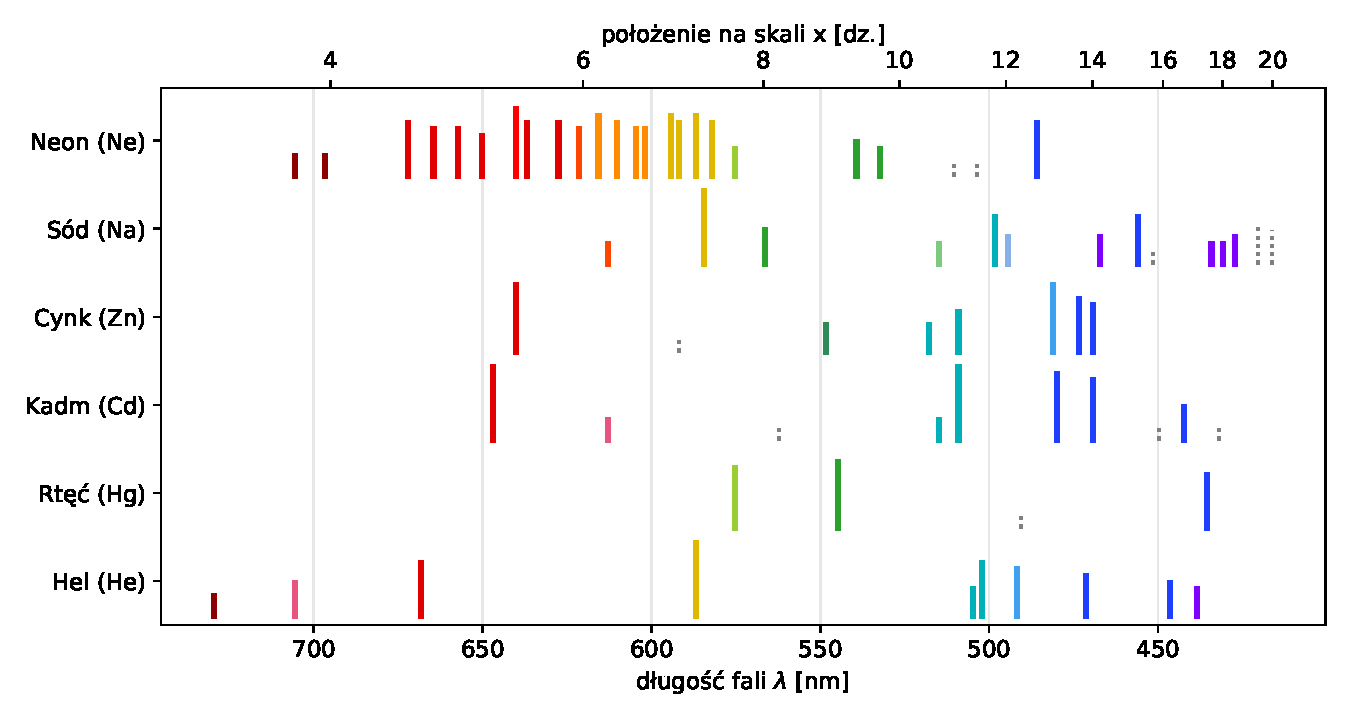
\includegraphics[width=0.95\textwidth]{spectra_calibrated.pdf}
    \caption{Widma wszystkich źródeł na skali długości fal, wyznaczonej z~krzywej dyspersji
             (górna oś --- odpowiadające położenie na skali spektroskopu). Linie odrzucone
             zaznaczono szarą linią przerywaną.}\label{fig:spectra_calibrated}
\end{figure}

\begin{table}[H]
    \centering
    \caption{Długości fal linii sodu wyznaczone z~krzywej dyspersji i~przypisane im dublety Na~I z~NIST~\cite{nist} (średnia składowych); $z = |\lambda - \lambda_\text{NIST}|/\sqrt{u^2(\lambda) + u_\lambda^2}$, $n_{2\sigma}$ --- liczba linii kandydujących w~odległości $\leq 2\sigma$.}\label{tab:sodium}
    \begin{tabular}{c S[table-format=2.1] S[table-format=3.1]@{\,$\pm$\,}S[table-format=1.1] S[table-format=3.3] S[table-format=+1.1] S[table-format=1.2] c}
        \toprule
        Nr & {$x$ [dz.]} & \multicolumn{2}{c}{$\lambda$ [nm]} & {$\lambda_\text{NIST}$ [nm]} & {$\lambda - \lambda_\text{NIST}$ [nm]} & {$z$} & $n_{2\sigma}$ \\
        \midrule
        1 & 6.4 & 612.9 & 5.9 & 615.749 & -2.9 & 0.48 & 1 \\
        2 & 7.5 & 584.4 & 5.0 & 589.294 & -4.9 & 0.97 & 1 \\
        3 & 8.3 & 566.4 & 4.5 & 568.542 & -2.1 & 0.47 & 1 \\
        4 & 11.2 & 514.9 & 3.2 & 515.112 & -0.2 & 0.07 & 1 \\
        5 & 12.4 & 498.1 & 2.8 & 498.068 & +0.1 & 0.03 & 1 \\
        7 & 15.1 & 467.2 & 2.1 & 466.668 & +0.6 & 0.26 & 1 \\
        8 & 16.3 & 455.8 & 1.9 & 454.341 & +1.5 & 0.77 & 1 \\
        10 & 19.0 & 434.1 & 1.7 & 434.311 & -0.2 & 0.12 & 2 \\
        11 & 19.5 & 430.6 & 1.7 & 428.942 & +1.6 & 0.97 & 3 \\
        12 & 20.0 & 427.2 & 1.7 & 427.521 & -0.3 & 0.18 & 2 \\
        \bottomrule
    \end{tabular}
\end{table}

Przypisano 10 z~11 linii sodu, wszystkie z~$z < 1$, a~dla 7 z~nich identyfikacja jest
jednoznaczna ($n_{2\sigma} = 1$). Dublet D wyznaczono jako $(584{,}4 \pm 5{,}0)$~nm wobec
$589{,}294$~nm ($z = 0{,}97$); różnica $-4{,}9$~nm jest największym odstępstwem wśród
linii niezależnych od kalibracji. Linię D zanotowano przy $7{,}5$~dz., a~linie He~I
$587{,}562$~nm i~Ne~I $588{,}189$~nm --- przy $7{,}4$ i~$7{,}2$~dz., więc trzy linie
z~przedziału 2~nm leżą na skali w~kolejności niezgodnej z~długością fali. Rozrzut
$0{,}3$~dz. jest porównywalny z~$u_x$, ale może też oznaczać przesunięcie skali między
pomiarami kolejnych źródeł. Odczytu kontrolnego położenia żółtej linii sodu, zalecanego
w~skrypcie~\cite{skrypt}, nie wykonano, więc stabilności skali nie można sprawdzić.
Linia Na~6 ($(494{,}3 \pm 2{,}7)$~nm,
Tabela~\ref{tab:unassigned}) nie ma odpowiednika w~widmie Na~I; najbliższa jest linia
Ne~I $495{,}703$~nm ($0{,}5\sigma$), której nie zaobserwowano jednak w~widmie rurki
z~neonem.

\begin{table}[H]
    \centering
    \small
    \caption{Długości fal linii neonu wyznaczone z~krzywej dyspersji i~przypisane im linie Ne~I z~NIST~\cite{nist}; $b$ --- zanotowana jasność, $I_\text{NIST}$ --- względna intensywność linii w~NIST, „stabilne” --- czy przypisanie jest takie samo dla każdego $\beta \in \{1, 2, 3, 4\}$. Pozostałe oznaczenia jak w~Tabeli~\ref{tab:sodium}.}\label{tab:neon}
    \begin{tabular}{c c S[table-format=2.1] S[table-format=3.1]@{\,$\pm$\,}S[table-format=2.1] S[table-format=3.3] S[table-format=6.0] S[table-format=+1.1] S[table-format=1.2] c c}
        \toprule
        Nr & $b$ & {$x$ [dz.]} & \multicolumn{2}{c}{$\lambda$ [nm]} & {$\lambda_\text{NIST}$ [nm]} & {$I_\text{NIST}$} & {$\lambda - \lambda_\text{NIST}$ [nm]} & {$z$} & $n_{2\sigma}$ & stabilne \\
        \midrule
        1 & 2 & 3.8 & 706 & 10 & 703.241 & 85000 & +2.4 & 0.23 & 7 & tak \\
        2 & 2 & 4.0 & 696.7 & 9.7 & 692.947 & 100000 & +3.8 & 0.39 & 5 & tak \\
        3 & 7 & 4.6 & 672.1 & 8.4 & 667.828 & 5000 & +4.3 & 0.51 & 5 & tak \\
        4 & 6 & 4.8 & 664.5 & 8.1 & 665.209 & 1500 & -0.7 & 0.08 & 7 & tak \\
        5 & 6 & 5.0 & 657.3 & 7.7 & 659.895 & 10000 & -2.6 & 0.34 & 9 & tak \\
        6 & 5 & 5.2 & 650.2 & 7.4 & 650.653 & 15000 & -0.4 & 0.06 & 11 & tak \\
        7 & 9 & 5.5 & 640.2 & 7.0 & 640.225 & 20000 & -0.1 & 0.01 & 17 & tak \\
        8 & 7 & 5.6 & 636.9 & 6.9 & 638.299 & 10000 & -1.4 & 0.20 & 17 & tak \\
        9 & 7 & 5.9 & 627.5 & 6.5 & 626.649 & 10000 & +0.9 & 0.13 & 20 & tak \\
        10 & 6 & 6.1 & 621.5 & 6.3 & 621.728 & 10000 & -0.2 & 0.03 & 19 & tak \\
        11 & 8 & 6.3 & 615.7 & 6.0 & 616.359 & 10000 & -0.7 & 0.11 & 14 & tak \\
        12 & 7 & 6.5 & 610.1 & 5.8 & 614.306 & 10000 & -4.2 & 0.72 & 14 & nie \\
        13 & 6 & 6.7 & 604.6 & 5.6 & 607.434 & 10000 & -2.8 & 0.50 & 13 & tak \\
        14 & 6 & 6.8 & 602.0 & 5.6 & 603.000 & 10000 & -1.0 & 0.19 & 12 & tak \\
        15 & 8 & 7.1 & 594.2 & 5.3 & 594.483 & 5000 & -0.3 & 0.05 & 12 & tak \\
        16 & 7 & 7.2 & 591.7 & 5.2 & 588.189 & 10000 & +3.5 & 0.68 & 12 & nie \\
        17 & 8 & 7.4 & 586.8 & 5.1 & 585.249 & 20000 & +1.6 & 0.31 & 10 & tak \\
        18 & 7 & 7.6 & 582.1 & 4.9 & 582.016 & 5000 & +0.0 & 0.01 & 10 & tak \\
        19 & 3 & 7.9 & 575.2 & 4.7 & 576.442 & 7000 & -1.3 & 0.27 & 8 & nie \\
        20 & 4 & 9.7 & 539.3 & 3.7 & 540.056 & 20000 & -0.8 & 0.21 & 12 & tak \\
        21 & 3 & 10.1 & 532.3 & 3.6 & 533.078 & 6000 & -0.8 & 0.21 & 8 & nie \\
        24 & 7 & 13.4 & 485.7 & 2.5 & 483.731 & 5000 & +2.0 & 0.80 & 15 & nie \\
        \bottomrule
    \end{tabular}
\end{table}

Przypisano wszystkie 22 linie neonu, z~$z \leq 0{,}80$ (Tabela~\ref{tab:neon}).
Najjaśniejszym liniom przypisano najsilniejsze linie Ne~I w~ich otoczeniu: Ne~7 (jasność 9)
--- $640{,}225$~nm, Ne~17 (jasność 8) --- $585{,}249$~nm. Każda linia ma jednak od 5 do 20
kandydatów w~odległości $2\sigma$, a~5 z~22 przypisań (Ne~12, 16, 19, 21 i~24) zmienia się
ze zmianą $\beta$, więc żadna identyfikacja nie jest jednoznaczna. Pięciu silnym liniom
Ne~I ($I_\text{NIST} \geq 10\,000$) z~obserwowanego zakresu nie przypisano żadnej linii.
Trzy z~nich ($702{,}405$, $633{,}443$ i~$534{,}109$~nm) leżą $1$--$5$~nm od linii przypisanych
($703{,}241$, $638{,}299$ i~$533{,}078$~nm), czyli $0{,}02$--$0{,}15$~dz. na skali, więc mogły
zlewać się z~nimi w~jedną linię. Linii $495{,}703$ i~$488{,}492$~nm nie zaobserwowano.

Dwie słabe linie lampy kadmowej, Cd~2 i~Cd~4, leżą dokładnie w~położeniach linii sodu
Na~1 i~Na~4 ($6{,}4$ i~$11{,}2$~dz.), co mogłoby wskazywać na domieszkę sodu. Tę możliwość
odrzucono: w~lampie kadmowej nie zaobserwowano linii D ($7{,}5$~dz.), najjaśniejszej
w~widmie lampy sodowej (jasność 10). Obie linie mają natomiast odpowiedniki w~widmie Cd~I
(Tabela~\ref{tab:cadmium}). Dla Cd~2 kandydatami są linie $609{,}914$~nm ($z = 0{,}50$)
i~$611{,}150$~nm ($z = 0{,}29$), więc identyfikacja jest niejednoznaczna. Dla Cd~4 jedynym
kandydatem jest linia $515{,}466$~nm ($z = 0{,}19$), ale ma ona $I_\text{NIST} = 6$, czyli
jest kilkadziesiąt do kilkuset razy słabsza od linii Cd~I użytych w~kalibracji
($I_\text{NIST} = 200$--$2000$). Zgodnie z~kryterium jasności stosowanym dla neonu
identyfikacja ta jest wątpliwa i~pochodzenie linii Cd~4 pozostaje niepewne.

\begin{table}[H]
    \centering
    \caption{Słabe linie lampy kadmowej nieużyte w~kalibracji i~przypisane im linie Cd~I z~NIST~\cite{nist}. Dla Cd~2 drugim kandydatem jest linia $611{,}150$~nm. Oznaczenia jak w~Tabelach~\ref{tab:sodium} i~\ref{tab:neon}.}\label{tab:cadmium}
    \begin{tabular}{c l S[table-format=2.1] S[table-format=3.1]@{\,$\pm$\,}S[table-format=1.1] S[table-format=3.3] S[table-format=3.0] S[table-format=1.2] c c}
        \toprule
        Nr & barwa & {$x$ [dz.]} & \multicolumn{2}{c}{$\lambda$ [nm]} & {$\lambda_\text{NIST}$ [nm]} & {$I_\text{NIST}$} & {$z$} & $n_{2\sigma}$ & stabilne \\
        \midrule
        2 & różowoczerwony (słaby) & 6.4 & 612.9 & 5.9 & 609.914 & 300 & 0.50 & 2 & nie \\
        4 & cyjan (słaby) & 11.2 & 514.9 & 3.2 & 515.466 & 6 & 0.19 & 1 & tak \\
        \bottomrule
    \end{tabular}
\end{table}

Różnice $\lambda - \lambda_\text{NIST}$ dla wszystkich porównywanych linii zestawiono na
Rysunku~\ref{fig:nist_comparison}.

\begin{figure}[H]
    \centering
    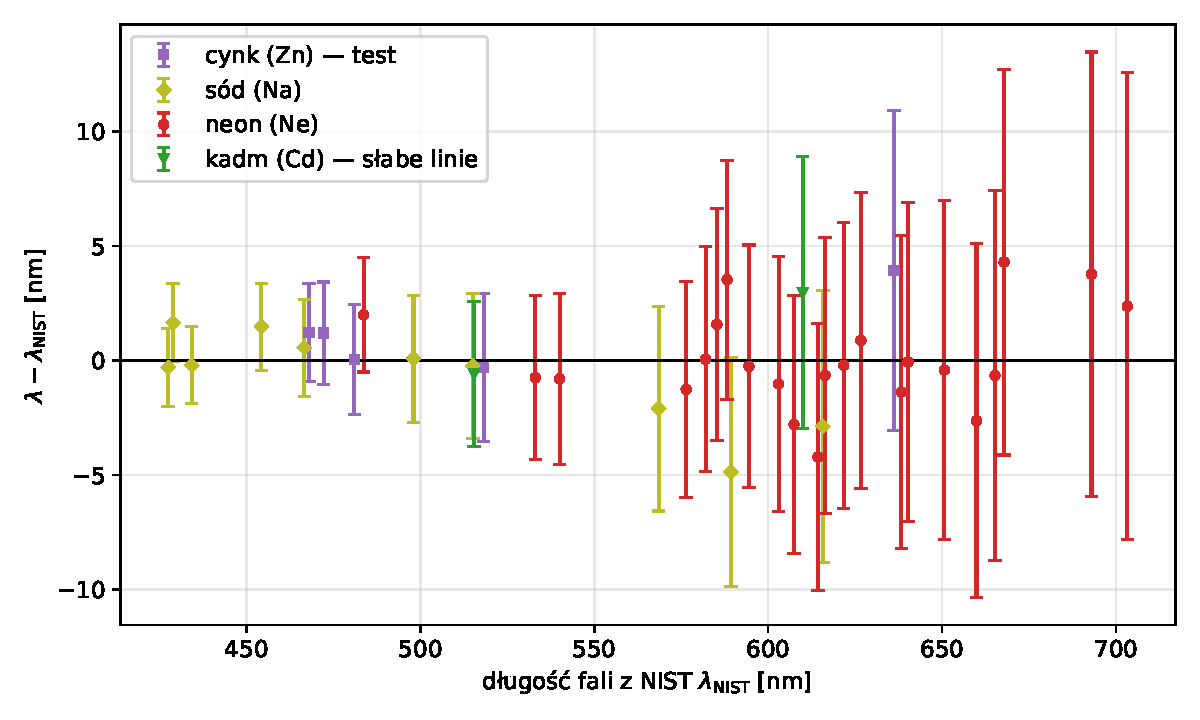
\includegraphics[width=0.78\textwidth]{nist_comparison.pdf}
    \caption{Różnica długości fali wyznaczonej z~krzywej dyspersji i~wartości z~NIST
             dla linii cynku (test), sodu, neonu i~słabych linii kadmu. Słupki błędów odpowiadają
             $\sqrt{u^2(\lambda) + u_\lambda^2}$.}\label{fig:nist_comparison}
\end{figure}



% -------------------------------------------
\section{Wnioski}
% -------------------------------------------

\subsection{Krzywa dyspersji}

Liniowa zależność $1/\lambda^2 = a_1 + a_2x$ ze skryptu nie opisuje krzywej dyspersji
spektroskopu na całym zakresie skali: $\chi^2/\nu = 2{,}16$ ($p \approx 0{,}004$),
a~na czerwonym końcu skali model odtwarza linię He $728{,}135$~nm jako $711{,}7$~nm.
Residua układają się w~łuk (Rysunek~\ref{fig:inverse_square}), czyli w~zależności
$1/\lambda^2(x)$ brakuje składowej kwadratowej. Jej współczynnik,
$a_3 = (-2{,}74 \pm 0{,}46)\cdot 10^{-3}$~\si{\micro\meter^{-2}}/dz.$^2$, różni się od zera
o~$6\sigma$, a~jego uwzględnienie obniża $\chi^2/\nu$ do $0{,}13$. Możliwymi źródłami tej
składowej są trzy przybliżenia, na których opiera się wzór~\eqref{eq:dispersion_linear}:
rozwinięcie $n(\delta)$ do pierwszego rzędu w~$\gamma$, liniowość odwzorowania kąta $\gamma$
na położenie na skali oraz dwuwyrazowy wzór Cauchy'ego (pominięty wyraz $C/\lambda^4$,
mierzalny np. dla szkieł flintowych). Każde z~nich daje poprawkę drugiego rzędu, więc
pomiar wyznacza jedynie ich łączny efekt $a_3$ i~nie pozwala ich rozróżnić.
Tak małe $\chi^2/\nu$ oznacza też, że przyjęta niepewność $u_x = 0{,}2$~dz. jest około
trzykrotnie większa od rzeczywistego rozrzutu odczytów ($0{,}066$~dz.), więc wszystkie
podane niepewności długości fal są zachowawcze.

\subsection{Linie cynku}

Długości fal pięciu linii cynku wyznaczone z~krzywej kwadratowej są zgodne z~wartościami
tablicowymi w~granicach niepewności, z~$z \leq 0{,}57$; najdokładniej wyznaczona linia
to $(481{,}1 \pm 2{,}4)$~nm wobec $481{,}053$~nm. Przy zawyżonych niepewnościach test
$3\sigma$ ma jednak małą moc --- przechodzi go także model liniowy. O~poprawności kalibracji
świadczy brak obciążenia: średnia różnica $\lambda - \lambda_\text{NIST}$ dla 12 linii
niezależnych od kalibracji (Zn i~jednoznacznie zidentyfikowane linie Na) wynosi
$(-0{,}2 \pm 1{,}4)$~nm dla modelu kwadratowego, wobec $(+2{,}2 \pm 1{,}3)$~nm dla modelu
liniowego, którego wszystkie wyniki dla Zn są przesunięte w~tę samą stronę. Ponieważ
obciążenie modelu liniowego na liniach niezależnych wynosi tylko $1{,}7\sigma$, wybór krzywej
kwadratowej opiera się na dopasowaniu do linii wzorcowych. Niepewność wyniku określa
niemal wyłącznie odczyt położenia ($88$--$91\,\%$ wariancji), a~w~czerwieni jest ona
trzykrotnie większa niż w~niebieskiej części widma z~powodu mniejszej dyspersji pryzmatu.

Linia lampy cynkowej przy $11{,}6$~dz., $(509{,}1 \pm 3{,}0)$~nm, wskazuje na domieszkę
kadmu: pokrywa się z~najsilniejszą linią Cd~I $508{,}582$~nm, a~położeniem i~barwą
z~linią Cd~5 lampy kadmowej. Pozostałe silne linie kadmu zlewają się z~liniami cynku. Linia przy $9{,}2$~dz.,
$(548{,}4 \pm 4{,}0)$~nm, może pochodzić od rtęci ($546{,}075$~nm), ale w~lampie cynkowej
nie zaobserwowano innych silnych linii Hg, więc pozostaje to hipotezą.

\subsection{Sód, neon i~słabe linie kadmu}

Wszystkie przypisane linie sodu są zgodne z~dubletami Na~I w~granicach niepewności,
w~tym dublet D, $(584{,}4 \pm 5{,}0)$~nm wobec $589{,}294$~nm. Dublet D odbiega najbardziej
spośród linii niezależnych, a~względem linii He i~Ne o~zbliżonej długości fali leży
w~odwróconej kolejności; bez odczytu kontrolnego nie da się rozstrzygnąć, czy to rozrzut
odczytu, czy przesunięcie skali. Siedem z~tych
identyfikacji jest jednoznacznych, więc widmo sodu stanowi drugi, niezależny test
kalibracji. Jedyna nieprzypisana linia sodu, $(494{,}3 \pm 2{,}7)$~nm, jest zgodna
z~linią Ne~I $495{,}703$~nm, której nie zaobserwowano jednak w~rurce z~neonem; w~widmie
sodu brak też najsilniejszej linii neonu ($640{,}225$~nm), więc pochodzenie Na~6
pozostaje nieustalone.

Słabe linie Cd~2 i~Cd~4 pokrywają się położeniem z~liniami Na~1 i~Na~4, ale domieszkę sodu
w~lampie kadmowej wyklucza brak linii D. Linia Cd~2 odpowiada linii Cd~I $609{,}914$ lub $611{,}150$~nm. Jedynym
kandydatem dla Cd~4 jest bardzo słaba linia Cd~I $515{,}466$~nm ($I_\text{NIST} = 6$),
więc pochodzenie Cd~4 pozostaje niepewne.

Po uwzględnieniu jasności najjaśniejszym liniom neonu przypisano najsilniejsze linie Ne~I
($640{,}225$ i~$585{,}249$~nm), a~wszystkie 22 linie są zgodne z~tablicą ($z \leq 0{,}80$).
Zgodność ta niewiele jednak mówi o~jakości kalibracji: w~czerwono-żółtej części widma
$u(\lambda)$ wynosi $5$--$10$~nm, a~linie Ne~I leżą co kilka nanometrów, więc w~przedziale
$2\sigma$ każdej linii mieści się od 5 do 20 kandydatów, a~5 przypisań zależy od wagi $\beta$,
więc identyfikacja poszczególnych linii zależy od przyjętego kryterium.

\begin{thebibliography}{9}
\bibitem{skrypt}
    \textit{Skrypt do I Pracowni Fizycznej}, ćwiczenie O10:
    Badanie widm emisyjnych za pomocą spektroskopu pryzmatycznego
\bibitem{nist}
    A.~Kramida, Yu.~Ralchenko, J.~Reader, NIST ASD Team,
    \textit{NIST Atomic Spectra Database},
    \url{https://physics.nist.gov/asd} [dostęp: 20 października 2026]
\end{thebibliography}

\end{document}
% =============================================
